
\vspace{-8mm}
\section{Introduction}
Large Language Models (LLMs) have achieved remarkable performance across various disciplines, including conversational AI and language translation. However, training and fine-tuning these models demand enormous computational resources and are highly memory-intensive. This substantial memory requirement arises not only from storing billions of trainable parameters but also from the need to store associated gradients and optimizer states—such as gradient momentum and variance in optimizers like Adam and AdamW—which can consume even more memory than the parameters themselves \citep{raffelExploringLimitsTransfer2020,touvronLlamaOpenFoundation2023,chowdheryPaLMScalingLanguage2022}.

To quantify this, consider a model with $\Psi$ parameters. Storing these parameters and their gradients in 16-bit precision formats like FP16 or BF16 requires $2\Psi$ bytes each. Optimizer states are typically stored in 32-bit precision (FP32) for numerical stability, necessitating an additional $4\Psi$ bytes for each of the parameters, gradient momentum and variance, amounting to $12\Psi$ bytes. Therefore, the total memory requirement sums up to $16\Psi$ bytes. When accounting for model-dependent memory such as activations during forward and backward passes, as well as residual memory like temporary buffers and memory fragmentation, the overall memory footprint can easily exceed $18\Psi$ bytes.

This enormous memory demand poses significant challenges, especially when training LLMs on hardware with limited memory capacity. As models continue to scale in size, efficient memory utilization becomes critical for making training feasible and accessible.

% 



\definecolor{cus_color}{rgb}{22, 96, 55}


\makeatletter
\newcommand{\removelatexerror}{\let\@latex@error\@gobble}
\makeatother


\begin{figure}[!t]
\centering
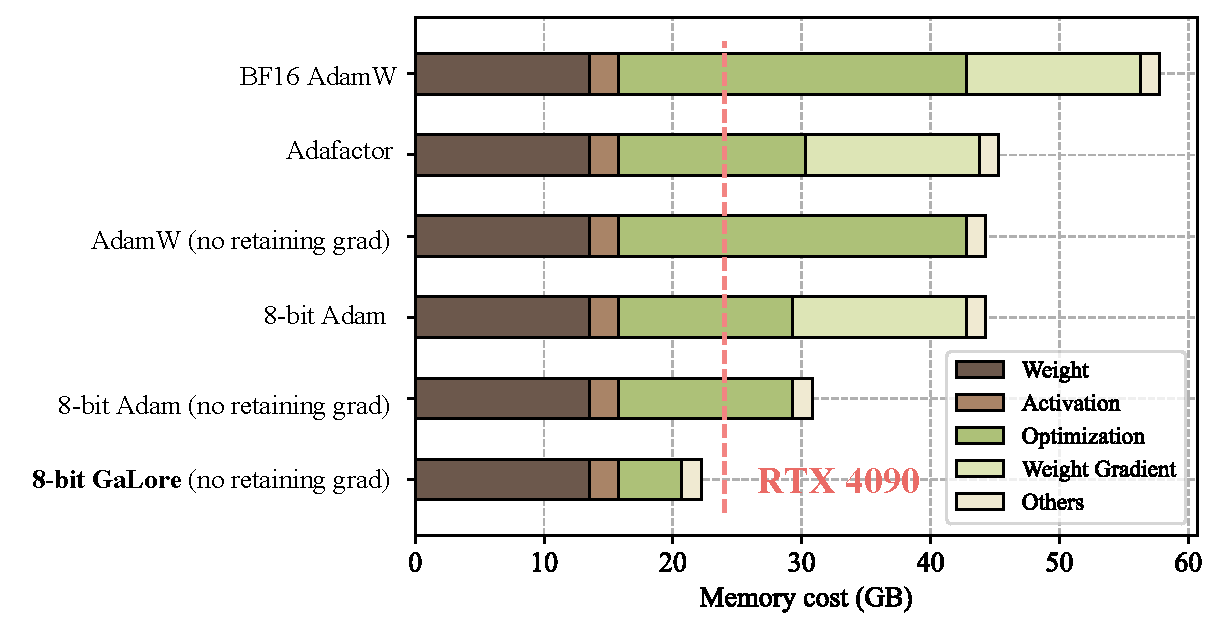
\includegraphics[width=1\columnwidth]{figures/files/memory_breakdown.pdf}
\vskip -0.11in
\caption{\small{Estimated memory consumption of pre-training a LLaMA 7B model with a token batch size of 256 on a single device, without activation checkpointing and memory offloading\protect\footnotemark[2]. Details refer to Section~\ref{sec:memory_measure}.}}
\label{fig:memory_breakdown} 
\vskip -0.15in
\end{figure}
\footnotetext[1]{The calculation is based on LLaMA architecture, BF16 numerical format, and maximum sequence length of 2048.}
\footnotetext[2]{In the figure, ``no retaining grad'' denotes the application of per-layer weight update to reduce memory consumption of storing weight gradient \citep{lvFullParameterFinetuning2023}.}
\SetAlFnt{\fontsize{8pt}{9pt}\selectfont}
\SetAlCapFnt{\fontsize{8pt}{9pt}\selectfont}
\begin{algorithm}[t]
    \SetAlgoLined
        \PyCode{for weight in model.parameters():} \\
        \Indp   %
            \PyCode{grad = weight.grad} \\ 
            \PyComment{original space -> compact space} \\
            \PyCode{lor\_grad = \textbf{project}(grad)} \\
            \PyComment{update by Adam, Adafactor, etc.} \\
            \PyCode{lor\_update = \textbf{update}(lor\_grad)} \\
            \PyComment{compact space -> original space} \\
            \PyCode{update = \textbf{project\_back}(lor\_update)} \\
            \PyCode{weight.data += update} \\
        \Indm %
    \caption{\fontsize{8pt}{9pt}\selectfont{\lowrank{}, PyTorch-like}}
    \label{alg:code_box}
\end{algorithm}


\paragraph{Parallel and Distributed Training Techniques}
To mitigate the substantial memory requirements in training large language models, researchers have developed various distributed computing techniques that leverage system-level optimizations and hardware resources. One prominent framework is \textbf{Distributed Data Parallel (DDP)} that combines \textbf{data parallelism} where the training dataset is partitioned across multiple devices or nodes, each holding a replica of the model with efficient gradient synchronization mechanisms, minimizing communication overhead. While data parallelism efficiently utilizes multiple GPUs, it can still face memory bottlenecks when model sizes exceed the memory capacity of a single device.

\textbf{Model parallelism} addresses this limitation by partitioning the model itself across multiple devices, allowing for the training of models that are too large to fit into the memory of a single GPU. Techniques like pipeline parallelism \citep{huangGPipeEfficientTraining2019} and tensor parallelism \citep{shoeybiMegatronLMTuningScaling2019} enable the distribution of different layers or partitions of layers across devices. However, model parallelism introduces communication overhead and can be complex to implement effectively.

Another effective technique is \textbf{gradient checkpointing} \citep{chenTrainingDeepNets2016}, which reduces memory usage by selectively storing only a subset of activations during the forward pass and recomputing them during the backward pass as needed. This approach trades increased computational overhead for reduced memory consumption, enabling the training of deeper models without exceeding memory constraints.

\textbf{Memory offloading strategies}, such as those implemented in ZeRO-Offload \citep{rajbhandariZeROMemoryOptimizations2020}, move optimizer states and gradients to CPU memory when not actively in use, freeing up GPU memory for other operations. The \textbf{Zero Redundancy Optimizer (ZeRO)} \citep{rajbhandariZeROMemoryOptimizations2020} further partitions optimizer states and gradients across data-parallel processes, eliminating redundancy and significantly reducing memory footprint. \textbf{Fully Sharded Data Parallel (FSDP)} \citep{zhaoExtendingTorchElasticStateful2020} extends this concept by sharding model parameters in addition to optimizer states and gradients.

 These system-level optimizations have been instrumental in training state-of-the-art LLMs such as LLaMA~1/2/3 \citep{touvronLlamaOpenFoundation2023}, GPT-3/4 \citep{brownLanguageModelsAre2020}, Mistral \citep{jiangMistralEfficientComposable2023}, and Gopher \citep{raeScalingLanguageModels2021} on multi-node, multi-GPU clusters.

While these distributed computing solutions enable the training of large models by leveraging extensive hardware resources, they come with increased system complexity and operational costs. Setting up and managing large-scale distributed training infrastructure can be challenging and may not be accessible to all researchers or organizations. Moreover, communication overhead and synchronization issues can impact training efficiency, particularly as models and datasets continue to grow in size.

Therefore, there is a pressing need for alternative approaches that reduce memory consumption without relying solely on distributed computing resources. Optimization techniques that approximate parameters or optimizer states, offer a promising direction for making LLM training more accessible and efficient.

\def\rr{\mathbb{R}}

\paragraph{Parameter-Efficient Fine-Tuning}

Parameter-Efficient Fine-Tuning (PEFT) techniques allow for the efficient adaptation of pre-trained language models to various downstream applications without the need to fine-tune all the model's parameters \citep{dingDeltaTuningComprehensive2022}. By updating only a small subset of parameters, PEFT methods significantly reduce the computational and memory overhead associated with full-model fine-tuning.

Among these techniques, the popular Low-Rank Adaptation (LoRA) \citep{huLoRALowRankAdaptation2021} \emph{reparameterizes} a weight matrix $W \in \mathbb{R}^{m \times n}$ as:
\begin{equation}
    W = W_0 + BA,
\end{equation}
where $W_0$ is a frozen full-rank pre-trained weight matrix, and $B \in \mathbb{R}^{m \times r}$ and $A \in \mathbb{R}^{r \times n}$ are trainable low-rank adapters to be learned during fine-tuning. Since the rank $r \ll \min(m, n)$, the adapters $B$ and $A$ contain significantly fewer trainable parameters, leading to reduced memory requirements for both parameter storage and optimizer states.

LoRA has been extensively used to reduce memory usage during fine-tuning, effectively enabling large models to be adapted to new tasks with minimal additional memory overhead. Its variant, ReLoRA \citep{lialinReLoRAHighRankTraining2023}, extends this approach to pre-training by periodically updating the frozen weight matrix $W_0$ using the previously learned low-rank adapters. This incremental updating allows for continual learning without the need to store full optimizer states for all parameters,leading to faster training times and lower computational costs. Furthermore, this allows for rapid adaptation of large models to multiple downstream tasks without the need to store separate copies of the entire model for each task.

There are a few variants of LoRA proposed to enhance its performance \citep{renduchintalaTiedLoraEnhacingParameter2023, shengSLoRAServingThousands2023, zhangLORAFAMEMORYEFFICIENTLOWRANK, xiaChainLoRAEfficient2024}, supporting multi-task learning \citep{wangMultiLoRADemocratizingLoRA2023}, and further reducing the memory footprint \citep{dettmersQLoRAEfficientFinetuning2023}.
\citet{lialinReLoRAHighRankTraining2023} proposed ReLoRA, a variant of LoRA designed for pre-training, but requires a full-rank training warmup to achieve comparable performance as the standard baseline. Inspired by LoRA, \citet{haoFloraLowRankAdapters2024} also suggested that gradients can be compressed in a low-rank subspace, and they proposed to use random projections to compress the gradients. There have also been approaches that propose training networks with low-rank factorized weights from scratch \citep{kamalakaraExploringLowRank2022,wangCuttlefishLowrankModel2023,zhaoInRankIncrementalLowRank2023}.

Despite their benefits, recent works have highlighted several limitations of low-rank reparameterization approaches. LoRA does not always achieve performance comparable to full-rank fine-tuning, particularly in complex tasks \citep{xiaChainLoRAEfficient2024}. In pre-training from scratch, methods like ReLoRA require an initial phase of full-rank model training as a warm-up before optimizing in the low-rank subspace \citep{lialinReLoRAHighRankTraining2023}.

These limitations may stem from inadequate low-rank approximation of the optimal weight matrices in large models, as well as altered training dynamics due to the reparameterization introduced by low-rank adapters. The shortcomings of low-rank parameter reparameterization suggest that alternative strategies are needed to achieve both memory efficiency and high performance.

\paragraph{Gradient Low-Rank Projection (GaLore)}

One promising direction is to approximate the \emph{optimizer states} instead of the parameters themselves. By reducing the memory footprint associated with optimizer states, it is possible to maintain full-parameter learning—thus preserving model capacity and performance—while still achieving significant memory savings.

The core idea behind GaLore is to harness the slowly changing low-rank structure of the \emph{gradient} matrix $G \in \mathbb{R}^{m \times n}$ corresponding to the weight matrix $W$, rather than approximating $W$ itself as a low-rank matrix. During neural network training, gradients naturally exhibit low-rank properties—a phenomenon studied extensively in both theoretical and practical settings \citep{zhaoZerOInitializationInitializing2022,cossonLowRankGradientDescent2023,yang2023spectral}. This intrinsic low-rank structure of gradients has been applied to reduce communication costs \citep{wangATOMOCommunicationefficientLearning,vogelsPowerGossipPracticalLowRank2020} and to decrease memory footprints during training \citep{gooneratneLowrankGradientApproximation2020,huangLowRankGradientDescent2023,modoranuErrorFeedbackCan2024}.

Specifically, GaLore computes two projection matrices $P \in \mathbb{R}^{m \times r}$ and $Q \in \mathbb{R}^{n \times r}$ to project the gradient matrix $G$ into a low-rank form:
\begin{equation}
    G_{\text{low-rank}} = P^\top G Q.
\end{equation}
Here, $r \ll \min(m, n)$ is the target rank, and $G_{\text{low-rank}}$ serves as an efficient approximation of the original gradient. The projection matrices $P$ and $Q$ are updated periodically (e.g., every 200 iterations) based on the principal components of recent gradients, which incurs minimal amortized computational cost.

By operating on low-rank approximations of the gradients, GaLore significantly reduces the memory footprint associated with storing optimizer states that rely on element-wise gradient statistics. In practice, this can yield up to \textbf{30\%} memory reduction compared to methods like LoRA during pre-training. Moreover, GaLore maintains full-parameter learning, allowing for updates to all model parameters, which can lead to better generalization and performance compared to low-rank adaptation methods. Further, GaLore is agnostic to the choice of optimizer and can be easily integrated into existing optimization algorithms with minimal code modifications.

While GaLore offers significant memory savings and enables full-parameter learning, its performance has not yet matched that of original optimizers like Adam or AdamW. Specifically, GaLore's reliance on low-rank gradient approximations can lead to suboptimal convergence rates and may not fully capture the rich optimization dynamics that these standard optimizers achieve with full gradients and optimizer states. These limitations suggest that while GaLore is a valuable step toward memory-efficient training, further enhancements are necessary to bridge the performance gap with standard optimizers.

\paragraph{Our Approach}

 To overcome the limitations of GaLore—particularly its performance gap with standard optimizers like Adam and AdamW—we introduce \textbf{Natural GaLore}. This method enhances GaLore by incorporating second-order information, specifically the curvature of the loss landscape, into the optimization process. By accounting for this curvature, Natural GaLore adjusts parameter updates more effectively, leading to faster convergence.

 Natural GaLore efficiently applies the inverse of the Empirical Fisher Information Matrix (FIM) to the low-rank gradients obtained from GaLore. Instead of computing and storing the full inverse FIM—which is computationally infeasible for large-scale models—we utilize the Woodbury Identity to perform this operation efficiently within the low-rank subspace. This approach allows us to incorporate second-order information without incurring significant computational or memory overhead.

 By integrating second-order information, Natural GaLore significantly improves the convergence rate, especially when the iteration budget is limited. This enhancement brings the performance of GaLore closer to that of standard optimizers like Adam or AdamW, effectively bridging the performance gap observed in previous methods.

 We validate the effectiveness of Natural GaLore through extensive empirical evaluations. Pre-training experiments on LLaMA models with 60M, 300M, and 1.1B parameters using the C4 dataset demonstrate that Natural GaLore achieves significantly lower perplexity compared to GaLore, all without additional memory overhead. This indicates that our method converges faster and reaches better optima within the same computational budget.

 Furthermore, we showcase the practical benefits of Natural GaLore in fine-tuning tasks. Specifically, we fine-tune the TinyLlama 1.1B model for function calling using the TinyAgent framework. Our results show that Natural GaLore significantly outperforms LoRA in this setting, achieving an accuracy of \textbf{83.5\%} on the TinyAgent dataset. This performance not only surpasses LoRA but also exceeds that of GPT-4o, which achieves \textbf{79.08\%} accuracy—all while using \textbf{30\%} less memory.

 In summary, Natural GaLore addresses the shortcomings of previous methods by efficiently incorporating second-order information into the optimization process. This leads to faster convergence rates and improved performance without additional memory requirements, making it a promising approach for training large-scale language models under memory constraints.




